\begin{figure}[ht!]
    \centering
    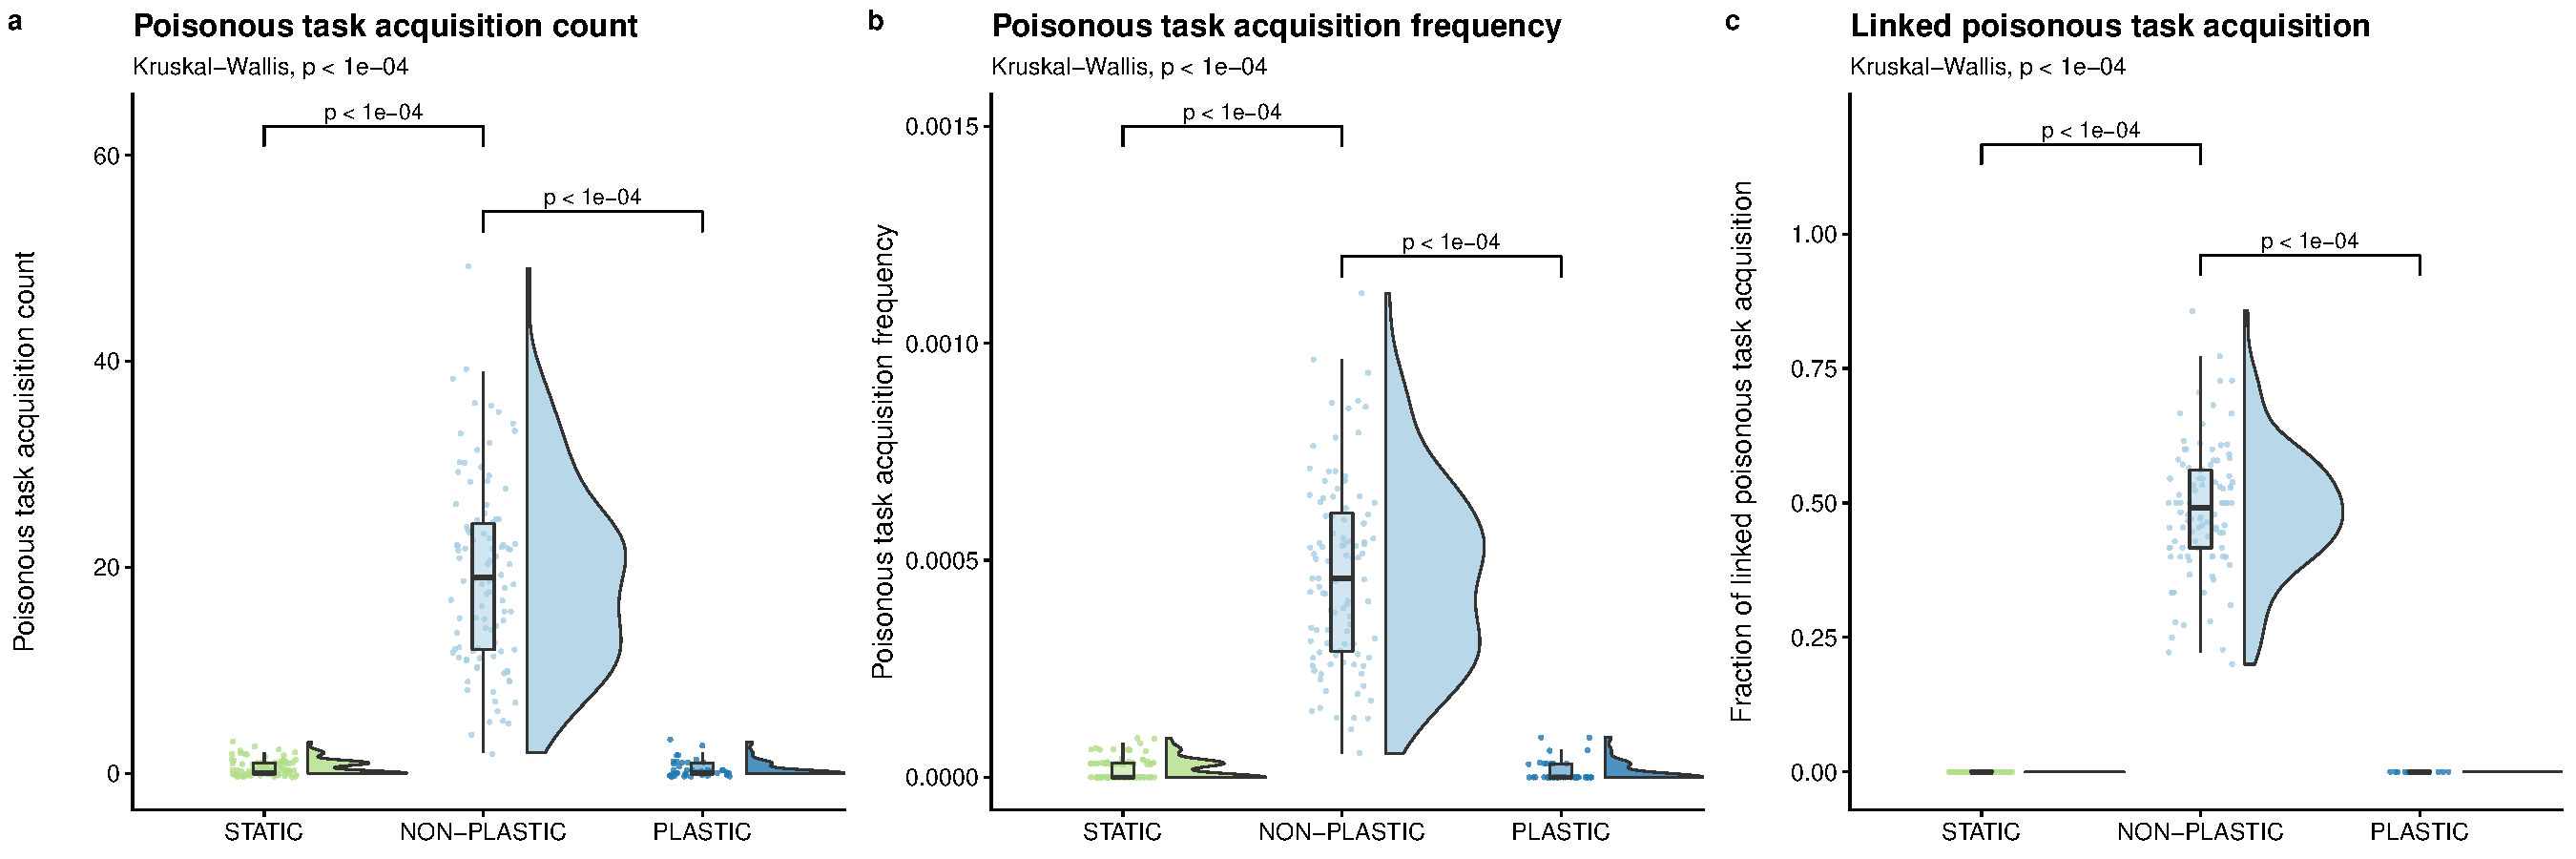
\includegraphics[width=1.0\textwidth]{chapters/03-evolutionary-consequences-of-plasticity/media/poison-accumulation-panel.pdf}
    \caption{\small
    \textbf{Deleterious instruction accumulation.}
    Raincloud plots of 
    (a) poisonous task acquisition,
    (b) poisonous task acquisition frequency,
    and (c) the proportion of mutations that increase poisonous task performance along a lineage that co-occur with a change in phenotypic profile.
    Each plot is annotated with statistically significant comparisons (Bonferroni-corrected pairwise Wilcoxon rank-sum tests).
    Note that adaptive phenotypic plasticity evolved in \deleteriousHitchhikingPlasticReps\ of \deleteriousHitchhikingReplicates\ replicates from the PLASTIC treatment during phase one of this experiment; 
    we used this more limited group to found \deleteriousHitchhikingPlasticReps\ phase-two PLASTIC replicates from which we report these PLASTIC data.
    }
    \label{chapter:consequences-of-plasticity:fig:deleterious-hitchhiking}
\end{figure}